%-------------------------------------------------------------------------
% Basic Compression Library Manual
%-------------------------------------------------------------------------

% Document class
\documentclass[a4paper,11pt,oneside]{report}

% Document title and API version
\newcommand{\bcldoctype}[1][0]{Manual}
\newcommand{\bclapiver}[1][0]{1.2}

% Common document settings and macros
%-------------------------------------------------------------------------
% Document formatting and macros for the Basic Compression Library manual
%-------------------------------------------------------------------------

% Misc. document info
\date{\today}

% Packages
\usepackage{fancyhdr}
\usepackage{lastpage}
\usepackage{listings}
\usepackage{color}
\usepackage[overload]{textcase}
\usepackage{times}
\usepackage{graphicx}

% Encoding
\usepackage[latin1]{inputenc}
\usepackage[T1]{fontenc}

% Page formatting
\usepackage[hmargin=2.5cm]{geometry}
\raggedright
\raggedbottom
\sloppy
\usepackage{parskip}

% Header and footer
\pagestyle{fancy}
\lhead{\textit{Basic Compression Library \bcldoctype}}
\chead{API version \bclapiver}
\rhead{Page \thepage/\pageref{LastPage}}
\lfoot{}
\cfoot{}
\rfoot{}
\renewcommand{\headrulewidth}{0.4pt}
\renewcommand{\footrulewidth}{0.0pt}

% Titlepage
\newcommand{\bclmaketitle}{\begin{titlepage}\ \\%
                           \begin{center}%
                           \vspace{7.0cm}{\Huge\textbf{Basic Compression Library}}\\%
                           \rule{10.0cm}{0.5pt}\\%
                           \vspace{0.5cm}{\LARGE\textbf{\bcldoctype}}\\%
                           \vspace{0.8cm}{\large\textbf{API version \bclapiver}}\\%
                           \textit{\today}\\%
                           \vspace{1.5cm}\textbf{\textcopyright2003-2006 Marcus Geelnard}\\%
                           \end{center}\end{titlepage}\newpage}

% Colors
\definecolor{code}{rgb}{0.9,0.9,1.0}
\definecolor{link}{rgb}{0.6,0.0,0.0}
\definecolor{codeA}{rgb}{0.9,1.0,0.9}
\definecolor{codeB}{rgb}{1.0,0.9,0.9}

% Code listings
\lstset{frame=single,frameround=tttt,backgroundcolor=\color{code},%
        language=C,basicstyle={\ttfamily},%
        breaklines,breakindent=0pt,postbreak=\space\space\space\space}

% hyperref (bookmarks, links etc) - use this package last
\usepackage[colorlinks=true,linkcolor=link,bookmarks=true,bookmarksopen=true,%
            pdfhighlight=/N,bookmarksnumbered=true,bookmarksopenlevel=1,%
            pdfview=FitH,pdfstartview=FitH]{hyperref}


% PDF specific document settings
\hypersetup{pdftitle={Basic Compression Library Manual}}
\hypersetup{pdfauthor={Marcus Geelnard}}
\hypersetup{pdfkeywords={Basic Compression Library,compression,Huffman,RLE,Rice,LZ77,Shannon-Fano,api,manual}}


%-------------------------------------------------------------------------
% Document body
%-------------------------------------------------------------------------

\begin{document}

\pagestyle{plain}

% Title page
\bclmaketitle

% Summary, trademarks and table of contents
\pagenumbering{roman}
\setcounter{page}{1}


%-------------------------------------------------------------------------
% Summary and Trademarks
%-------------------------------------------------------------------------
\chapter*{Summary}

This document describes the algorithms used in the Basic Compression Library,
and how to use the library interface functions.


%-------------------------------------------------------------------------
% Table of contents
%-------------------------------------------------------------------------
\tableofcontents


% Document chapters starts here...
\newpage
\pagenumbering{arabic}
\setcounter{page}{1}

\pagestyle{fancy}


%-------------------------------------------------------------------------
% Introduction
%-------------------------------------------------------------------------
\chapter{Introduction}
\thispagestyle{fancy}

\section{Background}
The Basic Compression Library is a set of open source implementations of
several well known lossless compression algorithms, such as Huffman and
RLE, written in portable ANSI C.

The library itself is not intended to serve as a competitor to advanced
general purpose compression tools, but rather as a reference or a set of
building blocks for custom compression algorithms.

An example of a field where customized compression algorithms can be be
useful is the compression of digitized media (such as images or audio),
for which you usually have lots of apriori information, and can tailor
an efficient method based on entropy reduction (e.g. differentiation)
followed by simple entropy coding (e.g. Huffman coding).

In many cases entropy reduction results in data that is NOT easily
compressed with advanced dictionary based general purpose entropy coders,
such as gzip or bzip2, since data often becomes very noisy after entropy
reduction. Even a simple Huffman coder can give better compression
results than the most advanced dictionary based coders under these
circumstances.


\section{The library philosophy}
All compression algorithms are represented by a coder and a decoder (a
compressor and a decompressor), often referred to as a CODEC.

All coders and decoders work on preallocated memory buffers, and do not
rely on any internal memory allocation or file I/O. In addition, all
library functions are 100\% reentrant.

No data integrity checking is performed within the library (e.g. there are
no CRCs stored in the compressed data streams, nor any information about
the size of the uncompressed data). This kind of functionality is left to
the user of the library.

The entire library is written in portable ANSI C code. The code should
work identically on 32-bit and 64-bit architectures, and on both little
endian and big endian systems (with the exception that the Rice
coder/decoder imports/exports data in machine native endian format).


%-------------------------------------------------------------------------
% The Compression Algorithms
%-------------------------------------------------------------------------
\chapter{The Compression Algorithms}
\thispagestyle{fancy}
This chapter briefly explains each compression algorithm, as it has been
implemented in the Basic Compression Library. For more in depth technical
information, see the source code and a decent resource on compression
algorithms.

\section{RLE}
RLE, or Run Length Encoding, is a very simple method for lossless
compression. It simply replaces repeated bytes with a short description
of which byte to repeat, and how many times to repeat it. Though simple
and obviously very inefficient fore general purpose compression, it can be
very useful at times (it is used in JPEG compression, for instance).

\subsection{Principle}
An example of how a run length encoding algorithm can encode a data
stream is shown in figure \ref{fig:rle}, where six occurrences of the symbol '93'
have been replaced with three bytes: a marker byte ('0' in this case),
the repeat count ('6'), and the symbol itself ('93').

\begin{figure}
\begin{center}
\begin{tabular}{|l|l|l|l|l|l|l|l|l|l|l|l|}\hline
12 & 65 & 14 & 52 & 53 & \emph{\textbf{93}} & \emph{\textbf{93}} & \emph{\textbf{93}} & \emph{\textbf{93}} & \emph{\textbf{93}} & \emph{\textbf{93}} & 32\\\hline
\end{tabular}

\ \\
\emph{...is encoded as...}
\\\ \\

\begin{tabular}{|l|l|l|l|l|l|l|l|l|}\hline
12 & 65 & 14 & 52 & 53 & \emph{\textbf{0}} & \emph{\textbf{6}} & \emph{\textbf{93}} & 32\\\hline
\end{tabular}
\end{center}
\caption{The principle of run lenght encoding.}
\label{fig:rle}
\end{figure}

When the RLE decoder encounters the symbol '0', which is used as the marker
byte, it will use the following two bytes to determine which symbol to output
and how many times to repeat the symbol.


\subsection{Implementation}
There are several different ways to do RLE. The particular method
implemented in the Basic Compression Library is a very efficient one.
Instead of coding runs for both repeating and non-repeating sections, a
special marker byte is used to indicate the start of a repeating section.
Non-repeating sections can thus have any length without being interrupted
by control bytes, except for the rare case when the special marker byte
appears in the non-repeating section (which is coded with at most two
bytes). For optimal efficiency, the marker byte is chosen as the least
frequent (perhaps even non-existent) symbol in the input stream.

Repeating runs can be as long as 32768 bytes. Runs shorter than 129
bytes require three bytes for coding (marker + count + symbol), whereas
runs longer than 128 bytes require four bytes for coding (marker +
counthi|0x80 + countlo + symbol). This is normally a win in compression,
and it is very seldom a loss of compression ratio compared to using a
fixed coding of three bytes (which allows coding a run of 256 bytes in
just three bytes).

With this scheme, the worst case compression result is:
$outsize=\frac{257}{256}\times insize+1$.


\section{Shannon-Fano}
\label{sec:shannonfano}
Shannon-Fano coding was invented by Claude Shannon (often regarded as
the father of information theory) and Robert Fano in 1949. It is a
very good compression method, but since David Huffman later improved the
method (see \ref{sec:huffman}), the original Shannon-Fano coding method
is almost never used. However, it is presented here for completeness.

The Shannon-Fano coding method replaces each symbol with an alternate
binary representation, whose length is determined by the probability of
the particular symbol. Common symbols are represented by few bits, while
uncommon symbols are represented by many bits.

The Shannon-Fano algorithm produces a very compact representation of
each symbol that is almost optimal (it approaches optimal when the number
of different symbols approaches infinite). However, it does not deal with
the ordering or repetition of symbols or sequences of symbols.


\subsection{Principle}
I will not go into all the practical details about Shannon-Fano coding, but
the basic principle is to find new binary representations for each
symbol so that common symbols use few bits per symbol, while uncommon
symbols use more bits per symbol.

The solution to this problem is, in short, to make a histogram of the
uncompressed data stream in order to find how common each symbol is.
A binary tree is then created by recursively splitting this histogram
in halves, where each half in each recursion should weigh as much as the
other half (the weight is $\sum_{k=1}^{N}{symbolcount_k}$, where $N$ is
the number of symbols in the branch and $symbolcount_k$ is the number of
occurrences of symbol $k$).

This tree serves two purposes:
\begin{enumerate}
\item The coder uses the tree to find the optimal representations for
      each symbol.
\item The \emph{de}coder uses the tree to uniquely identify the start
      and stop of each code in the compressed data stream: by traversing
      the tree from top to bottom while reading the compressed data
      bits, selecting branches based on each individual bit in the data
      stream, the decoder knows that a complete code has been read once
      a leaf node is reached.
\end{enumerate}

Let us have a look at an example to make it more clear. Figure
\ref{fig:huff1} shows an uncompressed data stream consisting of ten
bytes.

Based on the symbol frequencies, the Shannon-Fano coder comes up with the
Shannon-Fano tree (figure \ref{fig:huff3}) and the accompanying coded
representation (figure \ref{fig:huff2}).

As you can see, common symbols are closer to the root node (the top
of the figure), thus requiring fewer bits for representation. Based
on the found Shannon-Fano tree, the coder then encodes the data stream
with the alternate representation, as can be seen in \ref{fig:huff4}.

The total size of the compressed data stream is 24 bits (three bytes),
compared to the original 80 bits (10 bytes). Of course, we would have
to store the actual Shannon-Fano tree too so that the decoder is able to decode
the compressed stream, which would probably make the true size of the
compressed data stream \emph{larger} than the input stream in this
case. This is a side effect of the relatively short data set used in
this example. For larger data sets, the overhead of the Shannon-Fano tree
becomes negligible.

As an exercise, try decoding the compressed data stream by traversing
the Shannon-Fano tree from top to bottom, selecting left/right branches for
each new bit in the compressed data stream. Each time a leaf node is
encountered, the corresponding byte is written to the decompressed
output stream, and the tree traversal starts over from the root again.

\begin{figure}[p]
\begin{center}
\begin{tabular}{|l|l|l|l|l|l|l|l|l|l|}\hline
32 & 22 & 22 & 43 & 49 & 22 & 22 & 17 & 48 & 43\\\hline
\end{tabular}
\end{center}
\caption{Uncompressed data stream, used as input to the Shannon-Fano coder.}
\label{fig:huff1}
\end{figure}

\begin{figure}[p]
\begin{center}
\begin{tabular}{|r|r|l|}\hline
\textbf{Symbol} & \textbf{Frequency} & \textbf{Code}\\\hline
22 & 4 & 00\\\hline
43 & 2 & 01\\\hline
17 & 1 & 100\\\hline
32 & 1 & 101\\\hline
48 & 1 & 110\\\hline
49 & 1 & 111\\\hline
\end{tabular}
\end{center}
\caption{Symbol frequencies and encoding for the data stream in figure \ref{fig:huff1}.}
\label{fig:huff2}
\end{figure}

\begin{figure}[p]
\begin{center}
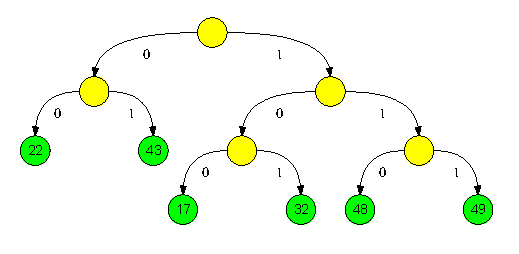
\includegraphics[width=15cm]{huffman_tree}
\end{center}
\caption{Shannon-Fano tree for the data stream in figure \ref{fig:huff1}.}
\label{fig:huff3}
\end{figure}

\begin{figure}[p]
\begin{center}
\begin{tabular}{|l|l|l|l|l|l|l|l|l|l|}\hline
101 & 00 & 00 & 01 & 111 & 00 & 00 & 100 & 110 & 01\\\hline
\end{tabular}
\end{center}
\caption{Compressed data stream.}
\label{fig:huff4}
\end{figure}


\subsection{Implementation}
The Shannon-Fano coder that can be found in the Basic Compression Library
is a very straight forward implementation. It is mostly included here for
the purpose of completeness.


\section{Huffman}
\label{sec:huffman}
The Huffman coding method was presented by David A. Huffman, a graduate
student of of Robert Fano, in 1952. Technically, it is very similar to the
Shannon-Fano coder (see \ref{sec:shannonfano}), but it has the nice
property of being optimal in the sense that changing any of the binary
codings of any of the symbols will result in a less compact representation.

The only real difference between the Huffman coder and the Shannon-Fano
coder is the way the binary coding tree is built: in the Shannon-Fano
method, the binary tree is built by recursively splitting the histogram
into equally weighted halves (i.e. top-down), while in the Huffman
method, the tree is built by succesively joining the two least weighing
nodes until there is only a single node left - the root node (i.e.
bottom-up).

Since Huffman coding has the same complexity as Shannon-Fano coding
(this also holds for decoding), but always compresses better, although
only slightly, Huffman coding is almost always used instead of Shannon-Fano
coding in reality.


\subsection{Principle}
As mentioned above, the principle of the Huffman coding method is very
similar to the Shannon-Fano coding method. The only difference lies in
how the binary tree is built.

In Huffman coding, the tree is built from the bottom up. Initially,
all leaf nodes are stored in a list, containing their symbol and weight
(proportional to the frequency of the specific symbol).

The tree is built by successively joyning the two least weighing nodes
in the list into a parent node. The parent node is assigned the sum of
the weights of the two child nodes. The child nodes are removed from the
list, and the parent node is added.

When there is only one node left in the tree, the process stops, and
the final node is the root node of the binary tree.

Writing and reading the coded data stream is done in exactly the same
way in Huffman coding as in Shannon-Fano coding.


\subsection{Implementation}
The Huffman coder that can be found in the Basic Compression Library is
a very straight forward implementation.

Primary flaws with this primitive implementation are:
\begin{itemize}
\item Slow bit stream implementation
\item Maximum tree depth of 32 (the coder aborts if any code exceeds a
      size of 32 bits). If I am not mistaking, this should not be possible
      unless the input buffer is larger than $2^{32}$ bytes, which is not
      supported by the coder anyway (max $2^{32}-1$ bytes can be specified with
      an unsigned 32-bit integer).
\end{itemize}

On the other hand, there are a few advantages of this implementation:
\begin{itemize}
\item The Huffman tree is stored in a very compact form, requiring only
      10 bits per symbol on average (for 8 bit symbols), meaning a maximum
      of 320 bytes overhead.
\item The code should be fairly easy to follow.
\end{itemize}

The Huffman coder does quite well in situations where the data is noisy,
in which case most dictionary based coders run into problems.


\section{Rice}
For data consisting of large words (e.g. 16 or 32 bits) and mostly low
data values, Rice coding can be very successful at achieving a good
compression ratio. This kind of data is typically audio or high dynamic
range images that has been pre-processed with some kind of prediction
(such as delta to neighboring samples).

Although Huffman coding should be optimal for this kind of data, it is not
a very suitable method due to several reasons (for instance, a 32-bit
word size would require a 16 GB histogram buffer to encode the Huffman
tree). Therefor a more dynamic approach is more appropriate for data that
consists of large words.

\subsection{Principle}
The basic idea behind Rice coding is to store as many words as possible
with less bits than in the original representation (just as with Huffman
coding). In fact, one can think of the Rice code as a fixed Huffman code
(i.e. the codes are not determined by the actual statistical content of
the data, but by the assumption that lower values are more common than
higher values).

The coding is very simple: Encode the value X with X '1' bits followed by
a '0' bit.

\subsection{Implementation}
There are some optimizations in the Rice implementation that can be
found in the Basic Compression Library:

\begin{enumerate}
\item The k least significant bits of each word are stored as is, and the
      N-k most significant bits are encoded with Rice coding. k is chosen as
      the average number of bits for the previous few samples in the stream.
      This usually makes the best use of the Rice coding, "hides" noise from
      the Rice coder, and does not result in very long Rice codes for signals
      with varying dynamic range.

\item If the rice code becomes longer than a fixed threshold, T, an
      alternate coding is used: output T '1' bits, followed by
      floor(log2(X-T)) '1' bits, and one '0' bit, followed by X-T (represented
      by the least significant floor(log2(X-T))-1  bits). This gives pretty
      efficient coding even for large values, and prevents ridiculously long
      Rice codes (in the worst case scenario, a single Rice code for a 32-bit
      word may become as long as $2^{32}$ bits, or 512 MB).

      If the threshold is set to 4, then the following is the resulting code
      table:

\begin{tabular}{|l|l|l|l|l|}\hline
\textbf{X} & \textbf{bin} & \textbf{Rice} & \textbf{Thresholded Rice} & \textbf{Difference}\\\hline
  0 & 00000 &   0                     & 0              & \\\hline
  1 & 00001 &   10                    & 10             & \\\hline
  2 & 00010 &   110                   & 110            & \\\hline
  3 & 00011 &   1110                  & 1110           & \\\hline
  4 & 00100 &   11110                 & 11110          & \\\hline
  5 & 00101 &   111110                & 111110         & \\\hline
  6 & 00110 &   1111110               & 11111100       &       +1 \\\hline
  7 & 00111 &   11111110              & 11111101       & \\\hline
  8 & 01000 &   111111110             & 1111111000     &       +1 \\\hline
  9 & 01001 &   1111111110            & 1111111001     & \\\hline
 10 & 01010 &   11111111110           & 1111111010     &       -1 \\\hline
 11 & 01011 &   111111111110          & 1111111011     &       -2 \\\hline
 12 & 01100 &   1111111111110         & 111111110000   & \\\hline
 13 & 01101 &   11111111111110        & 111111110001   &       -1 \\\hline
 14 & 01110 &   111111111111110       & 111111110010   &       -2 \\\hline
 15 & 01111 &   1111111111111110      & 111111110011   &       -3 \\\hline
 16 & 10000 &   11111111111111110     & 111111110100   &       -4 \\\hline
 17 & 10001 &   111111111111111110    & 111111110101   &       -5 \\\hline
 18 & 10010 &   1111111111111111110   & 111111110110   &       -6 \\\hline
 19 & 10011 &   11111111111111111110  & 111111110111   &       -7 \\\hline
 20 & 10100 &   111111111111111111110 & 11111111100000 &       -5 \\\hline
\end{tabular}

      As you can see, only two codes result in a worse representation with the
      threshold method used in this implementation. The rest of the codes
      result in shorter or equally short codes as for standard Rice coding.

\item In the worst case scenario, the output buffer may grow by several
      orders of magnitude compared to the input buffer. Therefor the Rice
      coder in this implementation aborts if the output becomes larger than
      the input by simply making a copy of the input buffer to the output
      buffer, with a leading zero byte (making the output at most one byte
      larger than the input).
\end{enumerate}



\section{Lempel-Ziv (LZ77)}
There are many different variants of the Lempel-Ziv compression scheme.
The Basic Compression Library has a fairly straight forward implementation
of the LZ77 algorithm (Lempel-Ziv, 1977) that performs very well, while
the source code should be quite easy to follow.

The LZ coder can be used for general purpose compression, and performs
exceptionally well for compressing text. It can also be used in
combination with the provided RLE and Huffman coders (in the order:
RLE, LZ, Huffman) to gain some extra compression in most situations.


\subsection{Principle}
The idea behind the Lempel-Ziv compression algorithm is to take the
RLE algorithm a few steps further by replacing sequences of bytes
with references to previous occurrences of the same sequences.

For simplicity, the algorithm can be thought of in terms of string
matching. For instance, in written text certain strings tend to
occur quite often, and can be represented by pointers to earlier
occurrences of the string in the text. The idea is, of course, that
pointers or references to strings are shorter than the strings
themselves.

For instance, in the previous paragraph the string ``\texttt{string}''
is quite common, and replacing all occurrences but the first of that
string with references would gain several bytes of saved storage.

A string reference is typically represented by:

\begin{itemize}
\item A unique marker.
\item An offset count.
\item A string length.
\end{itemize}

Depending on the coding scheme a reference can either have a fixed
length or a variable length. The latter is often preferred since that
allows the coder to trade reference size for string size (i.e. it may
be worth the increased size in the reference representation if the
string is long enough).


\subsection{Implementation}
One of the problems with LZ77 is that the algorithm requires
exhaustive string matching. For every single byte in the input data
stream, every previous byte in the stream has to be considered as a possible
starting point for a matching string, which means that the compressor is
very slow.

Another problem is that it is not very easy to tune the representation of 
a string reference for optimal compression. For instance, one has to decide
if all references and all non-compressed bytes should occur on byte
boundaries in the compressed stream or not.

The Basic Compression Library uses a very straight forward implementation
that guarantees that all symbols and references are byte aligned, thus
sacrificing compression ratio, and the string matching routines are not
very optimized (there are no caches, history buffers or other similar
tricks to gain speed), which means that the routines are \emph{very} slow.

On the other hand, the decompression routines are very simple and fast.

An attempt to speed up the LZ77 coder has been made, which uses an index
array that speeds up the string matching process by a fair amount. Still,
it is usually slower than any conventional compression program or library.%
\footnote{On a 2 GHz CPU, the compression speed is usually in the order of
300~KB/s, depending on how compressible the data is.}


%-------------------------------------------------------------------------
% Compiling
%-------------------------------------------------------------------------
\chapter{Compiling}
\thispagestyle{fancy}

There is a Makefile included for the GNU C compiler (gcc). Just run
\texttt{make} from the \texttt{src} directory, and you will get a file
called \texttt{libbcl.a}, which is a static link library that you can copy
to your compiler's \texttt{lib} directory. You may also want to copy the
.h files to your compiler's \texttt{include} directory.

The library has been compiled with gcc 3.3 under Linux without any
problems, and it should compile under any environment with gcc support
out of the box (e.g. Windows/MinGW, Mac OS X, DOS/DJGPP, etc).

To compile the Basic Compression Library with an alternate compiler, you
can either change the Makefile as appropriate, or simply add the .c/.h
files to your own project.


%-------------------------------------------------------------------------
% Library API Reference
%-------------------------------------------------------------------------
\chapter{Library API Reference}
\thispagestyle{fancy}

All functions act on input and output buffers, which contain any kind of
binary data. All sizes are given in number of bytes. The output buffer
usually has to be slightly larger than the input buffer, in order to
accommodate potential overhead if the input data is difficult to compress.

\section{RLE\_Compress}
Syntax:
\begin{lstlisting}
outsize = RLE_Compress(in,out,insize)
\end{lstlisting}

\begin{tabular}{ll}
outsize & Size of output buffer after compression\\
in      & Pointer to the input buffer (uncompressed data)\\
out     & Pointer to the output buffer (compressed data)\\
insize  & Size of input buffer
\end{tabular}

The output buffer must be able to hold $insize\times\frac{257}{256}+1$ bytes.


\section{RLE\_Uncompress}
Syntax:
\begin{lstlisting}
RLE_Uncompress(in,out,insize)
\end{lstlisting}

\begin{tabular}{ll}
in      & Pointer to the input buffer (compressed data)\\
out     & Pointer to the output buffer (uncompressed data)\\
insize  & Size of input buffer
\end{tabular}

The output buffer must be able to hold the entire uncompressed data
stream.


\section{SF\_Compress}
Syntax:
\begin{lstlisting}
outsize = SF_Compress(in,out,insize)
\end{lstlisting}

\begin{tabular}{ll}
outsize & Size of output buffer after compression\\
in      & Pointer to the input buffer (uncompressed data)\\
out     & Pointer to the output buffer (compressed data)\\
insize  & Size of input buffer
\end{tabular}

The output buffer must be able to hold $insize\times\frac{101}{100}+384$ bytes.


\section{SF\_Uncompress}
Syntax:
\begin{lstlisting}
SF_Uncompress(in,out,insize,outsize)
\end{lstlisting}

\begin{tabular}{ll}
in      & Pointer to the input buffer (compressed data)\\
out     & Pointer to the output buffer (uncompressed data)\\
insize  & Size of input buffer\\
outsize & Size of output buffer
\end{tabular}

The output buffer must be able to hold $outsize$ bytes.


\section{Huffman\_Compress}
Syntax:
\begin{lstlisting}
outsize = Huffman_Compress(in,out,insize)
\end{lstlisting}

\begin{tabular}{ll}
outsize & Size of output buffer after compression\\
in      & Pointer to the input buffer (uncompressed data)\\
out     & Pointer to the output buffer (compressed data)\\
insize  & Size of input buffer
\end{tabular}

The output buffer must be able to hold $insize\times\frac{101}{100}+320$ bytes.


\section{Huffman\_Uncompress}
Syntax:
\begin{lstlisting}
Huffman_Uncompress(in,out,insize,outsize)
\end{lstlisting}

\begin{tabular}{ll}
in      & Pointer to the input buffer (compressed data)\\
out     & Pointer to the output buffer (uncompressed data)\\
insize  & Size of input buffer\\
outsize & Size of output buffer
\end{tabular}

The output buffer must be able to hold $outsize$ bytes.


\section{Rice\_Compress}
Syntax:
\begin{lstlisting}
outsize = Rice_Compress(in,out,insize,format)
\end{lstlisting}

\begin{tabular}{ll}
outsize & Size of output buffer after compression (in bytes)\\
in      & Pointer to the input buffer (uncompressed data)\\
out     & Pointer to the output buffer (compressed data)\\
insize  & Size of input buffer (in bytes)\\
format  & Word format (see rice.h)
\end{tabular}

The output buffer must be able to hold $insize+1$ bytes.


\section{Rice\_Uncompress}
Syntax:
\begin{lstlisting}
Rice_Uncompress(in,out,insize,outsize,format)
\end{lstlisting}

\begin{tabular}{ll}
in      & Pointer to the input buffer (compressed data)\\
out     & Pointer to the output buffer (uncompressed data)\\
insize  & Size of input buffer (in bytes)\\
outsize & Size of output buffer (in bytes)\\
format  & Word format (see rice.h)
\end{tabular}

The output buffer must be able to hold $outsize$ bytes.


\section{LZ\_Compress}
Syntax:
\begin{lstlisting}
outsize = LZ_Compress(in,out,insize)
\end{lstlisting}

\begin{tabular}{ll}
outsize & Size of output buffer after compression\\
in      & Pointer to the input buffer (uncompressed data)\\
out     & Pointer to the output buffer (compressed data)\\
insize  & Size of input buffer
\end{tabular}

The output buffer must be able to hold $insize\times\frac{257}{256}+1$ bytes.


\section{LZ\_CompressFast}
Syntax:
\begin{lstlisting}
outsize = LZ_CompressFast(in,out,insize,work)
\end{lstlisting}

\begin{tabular}{ll}
outsize & Size of output buffer after compression\\
in      & Pointer to the input buffer (uncompressed data)\\
out     & Pointer to the output buffer (compressed data)\\
insize  & Size of input buffer\\
work    & Pointer to a temporary buffer (internal working buffer)
\end{tabular}

The output buffer must be able to hold $insize\times\frac{257}{256}+1$ bytes,
and the work buffer must be able to hold $insize+65536$ unsigned
integers.


\section{LZ\_Uncompress}
Syntax:
\begin{lstlisting}
LZ_Uncompress(in,out,insize)
\end{lstlisting}

\begin{tabular}{ll}
in      & Pointer to the input buffer (compressed data)\\
out     & Pointer to the output buffer (uncompressed data)\\
insize  & Size of input buffer
\end{tabular}

The output buffer must be able to hold the entire uncompressed data
stream.


%-------------------------------------------------------------------------
% License
%-------------------------------------------------------------------------
\chapter{License}
\thispagestyle{fancy}
Copyright \textcopyright\ 2003-2006 Marcus Geelnard

This software is provided 'as-is', without any express or implied
warranty. In no event will the authors be held liable for any damages
arising from the use of this software.

Permission is granted to anyone to use this software for any purpose,
including commercial applications, and to alter it and redistribute it
freely, subject to the following restrictions:

\begin{enumerate}
\item The origin of this software must not be misrepresented; you must not
   claim that you wrote the original software. If you use this software
   in a product, an acknowledgment in the product documentation would
   be appreciated but is not required.

\item Altered source versions must be plainly marked as such, and must not
   be misrepresented as being the original software.

\item This notice may not be removed or altered from any source
   distribution.
\end{enumerate}



\end{document}
